\chapter{Force-Guided Robot Alignment}
This chapter follows on from the previous chapter, we continue to demonstrate some technical solutions of system integration. On top of that, Forces and Torques (F/T) sensor will be included to discuss. Therefore, you can see the chapter as a operating manual when you simultaneously own a robot arm, an F/T sensor and an end effector. First of all, we explain why we will use F/T sensor in our project in section \ref{sec:pro def}. Furthermore, we introduce how to do gravity compensation in senction \ref{sec:grav compen}. Admittance control based on F/T sensor is described in section \ref{sec:adm ctrl}. Reference Frame Changing of F/T sensor is interpreted in section \ref{sec:rfc}. Last but not least, we discuss affection of setting admittance control parameters in section \ref{sec:affection}.
\section{Problem Definition}
\label{sec:pro def}
(Main cause of surgical failure)
(Peg in hole method based on F/T feedback)
(Modes: Doctor Dragging and self-alignment)
how to compensate the gravity affection in section \ref{sec:grav compen}; how to use admittance control in section with F/T sensor \ref{sec:adm ctrl}; and how to obtain the real force and torque values in the tool tip frame in section \ref{sec:rfc}
\section{Integration of F/T sensor}
\label{sec:grav compen}
\begin{figure}[htbp]
\begin{center}
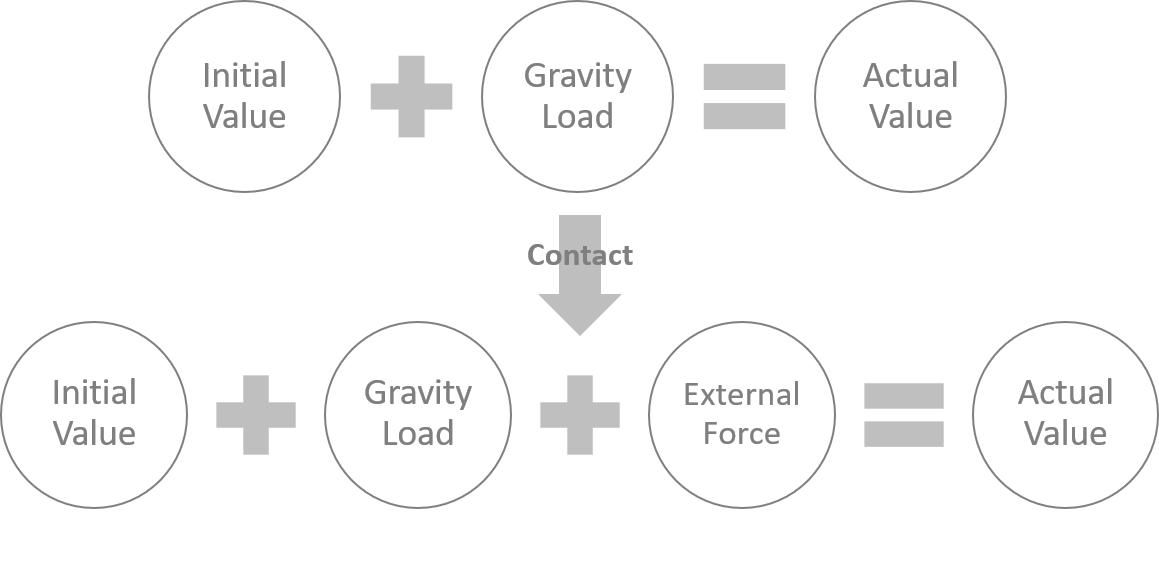
\includegraphics[width=1\linewidth]{Images/gravity compensation.png}
\end{center}
\caption{
Data Analysis of F/T sensor.
}\label{fig:gravity compensation}
\end{figure}
Gravity compensation is a critical technical issue when combining an F/T sensor with a robot arm and an end effector. Fundamentally, we should receive stable data when a static F/T sensor bears the same load or force. Nevertheless, our F/T sensor is installed on the robot arm and move with the pose of the robot arm. On account of its mobility, the gravity of the end effector will significantly affect the actual value we received. Moreover, starting without resetting the F/T sensor to zero would lead to an initial value. If we could not analyze the actual value to an initial value and a gravity load, we would obtain an unstable actual value, not to mention obtain the external force caused by contact force.

Therefore, we illustrate a method, which is to analyze the actual value of the F/T sensor to an initial value and gravity load in real-time. It's worth noting that with this approach, we can get the installation angle between the F/T sensor and the robot arm including assembly error, and we no longer need to reset the F/T sensor to zero every time.
\subsubsection{The Centroid Position of End Effector}
To start with the first equation in Figure \ref{fig:gravity compensation},
\begin{equation}\label{eq:gc_iga}
\begin{split}
\text{Initial value}	+ \text{Gravity Load} 		= \text{Actual Value} \\
\Rightarrow \left\{\begin{matrix}
\boldsymbol{f_0}		+\boldsymbol{f_g}			&= \boldsymbol{f}\\ 
\boldsymbol{\tau_0}	+\boldsymbol{\tau_g}		&= \boldsymbol{\tau}	
\end{matrix}\right.\Rightarrow \left\{\begin{matrix}
f_{0x} 				+f_{gx} 			&= f_x\\ 
f_{0y}				+f_{gz} 			&= f_y\\ 
f_{0z}				+f_{gy} 			&= f_z\\ 
\tau_{0x}			+\tau_{gx} 			&=\tau _x\\ 
\tau_{0y}			+\tau_{gy} 			&=\tau _y \\ 
\tau_{0z}			+\tau_{gz} 			&=\tau _z 
\end{matrix}\right.	\\
\end{split}
\end{equation}
where $\boldsymbol{f}$ and $\boldsymbol{\tau}$ are force and torque vector respectively.\\
And, by terms of moment arm formula,
\begin{equation}
\begin{split}
\because
\boldsymbol{\tau_g}	&= \boldsymbol{r} \times \boldsymbol{f_g} \\
\end{split}
\end{equation}

where $\boldsymbol{r}$ denotes the centroid position of the end effector in the sensor frame.
\begin{equation}
\begin{split}
\therefore\ 
\boldsymbol{\tau}		&= \boldsymbol{\tau_0}	+\boldsymbol{\tau_g}\\
						&= \boldsymbol{\tau_0}	+
						   \boldsymbol{r} \times \boldsymbol{f_g}\\
\end{split}
\end{equation}
Then, Substitute the first line of Equation \ref{eq:gc_iga} into the above equation, we will obtain
\begin{equation}
\begin{split}
\boldsymbol{\tau}	&=  \boldsymbol{\tau_0}+ 
						\boldsymbol{p}	\times \left( \boldsymbol{f} - \boldsymbol{f_0} \right) 
\end{split}
\end{equation}
, which could be extended as
\begin{equation}
\begin{split}
\left\{\begin{matrix}
\tau _{x}	=	\tau _{0x} 	+ \left( f_z - f_{0z}\right) \cdot y - \left( f_y - f_{0y}\right) \cdot z\\
\tau _{y}	=	\tau _{0y}	+ \left( f_x - f_{0x}\right) \cdot z - \left( f_z - f_{0z}\right) \cdot x\\
\tau _{z}	=	\tau _{0z}	+ \left( f_y - f_{0y}\right) \cdot x - \left( f_x - f_{0x}\right) \cdot y& 
\end{matrix}\right.	\\
\end{split}
\end{equation}
and be overwritten as
\begin{equation}\label{eq:matrix_mfrk}
\begin{split}
\begin{bmatrix}
\tau _x\\
\tau _y\\
\tau _z
\end{bmatrix}
=
\begin{bmatrix}
0		&f_z	&-f_y	&1	&0	&0\\
-f_z	&0		&f_x	&0	&1	&0\\
f_y		&-f_x	&0		&0	&0	&1
\end{bmatrix}
\begin{bmatrix}
x\\
y\\
z\\
k_1\\
k_2\\
k_3
\end{bmatrix}\\
\end{split}
\end{equation}

where
\begin{equation}\label{eq:k1k2k3}
\begin{split}
\left\{\begin{matrix}
k_1 = \tau _{0x} - \left( f_{0z} \cdot y + f_{0y} \cdot z \right)  &  \\
k_2 = \tau _{0y} - \left( f_{0x} \cdot z + f_{0z} \cdot x \right)  &\text{are all constant} \\
k_3 = \tau _{0z} - \left( f_{0y} \cdot x + f_{0x} \cdot y \right)  & 
\end{matrix}\right.\\
\end{split}
\end{equation}
With extracting $[x,y,z,k_1,k_2,k_3]$ in mind, we move the robot arm to $n\ (n\geq3)$ positions with different poses. By recording $n$ torque vector and corresponding $n$ force vector from F/T sensor, we can expand Equation \ref{eq:matrix_mfrk} as
\begin{equation}
\begin{split}
\begin{bmatrix}
\tau _{1x}\\
\tau _{1y}\\
\tau _{1z}\\
\tau _{2x}\\
\tau _{2y}\\
\tau _{2z}\\
\vdots\\
\tau _{nx}\\
\tau _{ny}\\
\tau _{nz}\\
\end{bmatrix}
=
\begin{bmatrix}
0			&f_{1z}		&-f_{1y}	&1	&0	&0\\
-f_{1z}		&0			&f_{1x}		&0	&1	&0\\
f_{1y}		&-f_{1x}	&0			&0	&0	&1\\
0			&f_{2z}		&-f_{2y}	&1	&0	&0\\
-f_{2z}		&0			&f_{2x}		&0	&1	&0\\
f_{2y}		&-f_{2x}	&0			&0	&0	&1\\
 			& 			&\vdots		& 	& 	& \\
0			&f_{nz}		&-f_{ny}	&1	&0	&0\\
-f_{nz}		&0			&f_{nx}		&0	&1	&0\\
f_{ny}		&-f_{nx}	&0			&0	&0	&1
\end{bmatrix}
\begin{bmatrix}
x\\
y\\
z\\
k_1\\
k_2\\
k_3
\end{bmatrix}\\
\end{split}
\end{equation}

, which is defined as 
\begin{equation}
\begin{split}
\boldsymbol{m}_{\left(3n \times 1\right)} = \mathbf{F}_{\left(3n \times 6\right)} \cdot \boldsymbol{p}_{\left(6 \times 1\right)}
\end{split}
\end{equation}
As a consequence of the full column rank of $\mathbf{F}$, we can apply Moore-Penrose pseudoinverse. Then, 
\begin{equation*}
\begin{split}
\boldsymbol{p} 	&= \mathbf{F}^{\dagger} \cdot \boldsymbol{m}\\
				&= \left( \mathbf{F}^\top\mathbf{F}\right) ^{-1}\mathbf{F}^\top \cdot \boldsymbol{m}
\end{split}
\end{equation*}

From now on, we have already known the centroid position of end effector in the sensor frame and values of the constants $k_1,k_2,k_3$.
\subsubsection{Gravity Compensation and Initial Value Reset}
Next, let us come back to the first equation in Figure \ref{fig:gravity compensation}. We continue to use this formula and contemplate it from the perspective of coordinate transformation relation. Here we hypothesize that the end effector weighs $g$ kilograms relative to the frame\{0\} which is also the world frame. That means the gravity vector of the end effector $\boldsymbol{^0\!g}$ is $[0,0,-g]$ in the frame\{0\}. Then, we can derive it as following.
\begin{equation}
\begin{split}
\text{Initial value}	+ \text{Gravity Load} 		&= \text{Actual Value} \\
\Rightarrow
\boldsymbol{f_0} +\  ^\mathrm{S}_6\mathbf{R} \cdot ^6_0\!\mathbf{R} \cdot \boldsymbol{^0\!g} &= \boldsymbol{f}
\end{split}
\end{equation}

which is relative to frame \{6\}.
Hence, we assume an installation angle $\theta$ including assembly error.
\begin{equation}
\begin{split}
 ^\mathrm{S}_6\mathbf{R}
=
\begin{bmatrix}
\cos(\theta)	&\sin(\theta)	&0 \\
-\sin(\theta)	&\cos(\theta)	&0 \\
0				&0				&1
\end{bmatrix}
\end{split}
\end{equation}
Besides, we can easily calculate $^6_0\mathbf{R}$ from Equation \ref{eq:translation matrix}.
\begin{equation}
\begin{split}
^6_0\mathbf{R} 	&=\ ^0_6\mathbf{R}^\top\\
				&\coloneqq
\begin{bmatrix}
r_{11}		&r_{12}		&r_{13} \\
r_{21}		&r_{22}		&r_{23} \\
r_{31}		&r_{32}		&r_{33}
\end{bmatrix}
\end{split}
\end{equation}
Therefore,
\begin{equation}
\begin{split}
\begin{bmatrix}
f_{0x}\\
f_{0y}\\
f_{0z}
\end{bmatrix}
+
\begin{bmatrix}
\cos(\theta)	&\sin(\theta)	&0 \\
-\sin(\theta)	&\cos(\theta)	&0 \\
0				&0				&1
\end{bmatrix}
\begin{bmatrix}
r_{11}		&r_{12}		&r_{13} \\
r_{21}		&r_{22}		&r_{23} \\
r_{31}		&r_{32}		&r_{33}
\end{bmatrix}
\begin{bmatrix}
0\\
0\\
-g
\end{bmatrix}
=
\begin{bmatrix}
f_x\\
f_y\\
f_z
\end{bmatrix}
\end{split}
\end{equation}

Further, we rewrite it as 
\begin{equation}
\begin{split}
\begin{bmatrix}
-r_{13}		&-r_{23} 	&0			&1		&0		&0\\
-r_{23}		&r_{13}		&0			&0		&1		&0\\
0			&0			&-r_{33}	&0		&0		&1
\end{bmatrix}
\begin{bmatrix}
g\cos(\theta)\\
g\sin(\theta)\\
g\\
f_{0x}\\
f_{0y}\\
f_{0z}
\end{bmatrix}
=
\begin{bmatrix}
f_x\\
f_y\\
f_z
\end{bmatrix}
\end{split}
\end{equation}
In the same way as Equation \ref{eq:matrix_mfrk}, we can extract $[g\cos(\theta),g\sin(\theta),g,f_{0x},f_{0y},f_{0z}]$ by the least square solution. Apparently, we can directly obtain $g,f_{0x},f_{0y},f_{0z}$. Afterwards, we substitute them into Equation \ref{eq:k1k2k3} to calculate 
\begin{equation}
\begin{split}
\left\{\begin{matrix}
\tau _{0x}	=	k_1	+ \left( f_{0z} \cdot y + f_{0y} \cdot z \right) \\
\tau _{0y} 	=	k_2	+ \left( f_{0x} \cdot z + f_{0z} \cdot x \right) \\
\tau _{0z} 	=	k_3 + \left( f_{0y} \cdot x + f_{0x} \cdot y \right)
\end{matrix}\right.\\
\end{split}
\end{equation}
Finally, we successfully obtain the weight of the end effector $g$, the initial value of the F/T sensor $[f_{0x},f_{0y},f_{0z},\tau_{0x},\tau_{0y},\tau_{0z}]$.

As for installation angle $\theta$ including assembly error,  there is an further discussion. Undoubtedly, we can derive it as
\begin{equation}
\begin{split}
\theta = \cos^{-1}\left(\frac{g\cos(\theta)}{g}\right)\ \text{or} \ \sin^{-1}\left(\frac{g\sin(\theta)}{g}\right)\
\end{split}
\end{equation}
In theory, By either arccos function or arcsin function we can derive the same value. However, we estimate $[g\cos(\theta),g\sin(\theta),g,f_{0x},f_{0y},f_{0z}]$ by using the least square solution which produce a approximated answer rather than the correct answer. A subtle bias caused by the least square solution will be enlarged through the arc function. 
Thankfully, we originally designed an adapter to connect the robot arm and F/T sensor and the installation angle is exactly zero degree. Therefore, here we only need to concern about the subtle bias result from assembly errors.\\
For example, here we compare arccos and arcsin with the same biases.
\begin{table}[htbp]
\centering
\caption{Arc-function Comparison}
\label{tab:arc}
\begin{tabular}{c|c|c} 
\hline \hline
bias $n$ (rad)	&$\sin^{-1}(n)$	(degree)	&$\cos^{-1}(1-n)$ (degree)\\
\hline
0				&0							&0\\
0.001			&0.057						&2.56\\
0.01			&0.57						&8.11\\
0.1				&5.7						&25.84
\end{tabular}
\end{table}
Obviously, if we separately give the same bias ( $0.1$ rad) into arccos and arcsin function, arccos function will enlarge the bias significantly larger than arcsin function. Hence we should use
\begin{equation}
\begin{split}
\theta = \sin^{-1}\left(\frac{g\sin(\theta)}{g}\right)\
\end{split}
\end{equation}
Notably, as a result of the zero installation angle which we originally designed, from Table \ref{tab:arc} we could infer to use arcsin function. In contrast, if the installation angle is not zero, the above assumption will be invalid.

Ultimately, we have successfully dissected the actual value of F/T sensor into the initial value of F/T sensor and the gravity of the end effector. 
\subsubsection{External Force Evaluation}
Next, we continue to review the second equation in  Figure \ref{fig:gravity compensation}.
\begin{equation}
\begin{split}
\text{Initial value}	+ \text{Gravity Load} 		+ \text{External Force}		&= \text{Actual Value} \\
\Rightarrow \left\{\begin{matrix}
\boldsymbol{f_0}		+\boldsymbol{f_g}		+\boldsymbol{f_e}		&= \boldsymbol{f}\\ 
\boldsymbol{\tau_0}		+\boldsymbol{\tau_g}	+\boldsymbol{\tau_e}		&= \boldsymbol{\tau}	
\end{matrix}\right.	\\
\end{split}
\end{equation}
Therefore,
\begin{equation}
\begin{split}
\boldsymbol{f_e}		&= \boldsymbol{f} 		- \boldsymbol{f_0}		-\boldsymbol{f_g}\\
						&= \boldsymbol{f} 		- \boldsymbol{f_0}		- ^\mathrm{S}_6\mathbf{R} \cdot ^6_0\!\mathbf{R} \cdot \boldsymbol{^0\!g}\\
\boldsymbol{\tau_e}		&= \boldsymbol{\tau}	- \boldsymbol{\tau_0}		-\boldsymbol{\tau_g}\\
						&= \boldsymbol{\tau}	- \boldsymbol{\tau_0}		-\boldsymbol{r} \times \boldsymbol{f_g}
\end{split}
\end{equation}
\begin{equation*}
\begin{split}
\Rightarrow 
\left\{\begin{matrix}
f_{ex} = f_x - f_{0x} 	+ g\cos(\theta)r_{13} 	+ g\sin(\theta)r_{23}\\
f_{ey} = f_y - f_{0y} 	- g\sin(\theta)r_{13} 	+ g\cos(\theta)r_{23}\\
f_{ez} = f_z - f_{0z} 	+ gr_{33}\\
\tau_{ex} = f_x - \tau_{0x} - \left( g_z\cdot y - g_y\cdot z \right)\\
\tau_{ey} = f_y - \tau_{0y} - \left( g_x\cdot z - g_z\cdot x \right)\\
\tau_{ez} = f_z - \tau_{0z} - \left( g_y\cdot x - g_x\cdot y \right)
\end{matrix}\right.
\end{split}
\end{equation*}
\section{Alignment to the Root Canal (Dragging for alignment)}
In the hope that dentist could drag our system to the infected teeth by holding the end effector, we usher in admittance control based on F/T sensor.
\subsection{Admittance Control based on F/T sensor}
Admittance control make the robot move like a spring-mass-damper system. Forces and torques can be mapped into the movements such as position or velocity. Most important of all, admittance control enables an robot arm to cooperate with human in a safe work environment.Since Meca500 is an industrial robot arm without admittance control, we subsequently combine the robot arm with the F/T sensor so as to adopt admittance control. With force and torque feedback, F/T sensor make Meca500 be resemble to a collaborative robot arm. Therefore, we propose a control scheme depicted as Figure \ref{fig:adm ctrl}. It's worth noting that in this approach the admittance control function is triggered by the end effector mounted on F/T sensor instead of detecting each wrist torque of the robot arm.

\label{sec:adm ctrl}
\begin{figure}[htbp]
\begin{center}
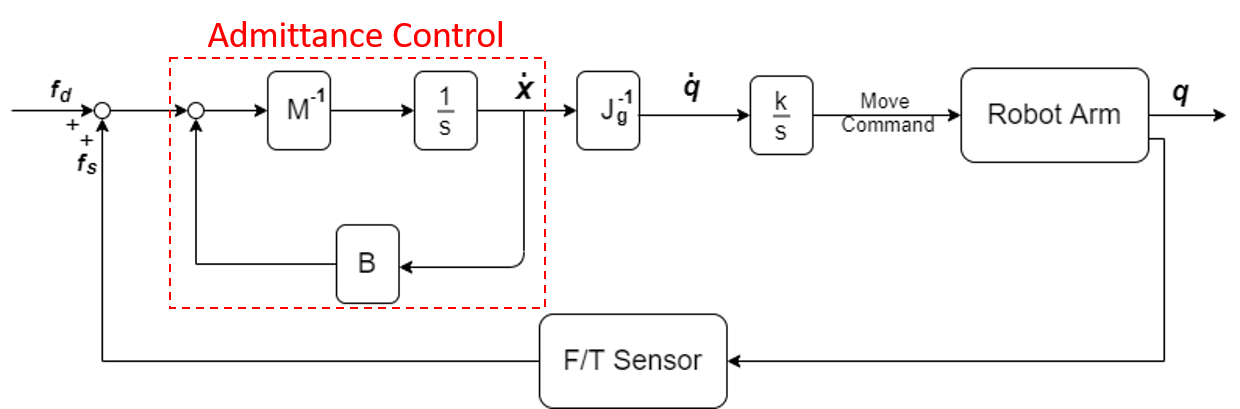
\includegraphics[width=1\linewidth]{Images/adm ctrl.png}
\end{center}
\caption{
Control scheme. $\boldsymbol{f_d}$ denotes the desired forces and torques vector. $\boldsymbol{f_s}$ denotes the real value detected by F/T sensor and is also a forces and torques vector. $\boldsymbol{\dot{x}}$ denotes [$\dot{x}, \dot{y}, \dot{z}, \dot{\theta _x}, \dot{\theta _y}, \dot{\theta _z}$]. $\mathbf{J_g}$ denotes the geometric Jacobian matrix. $\boldsymbol{\dot{q}}$ denotes [$\dot{\theta _1}, \dot{\theta _2}, \dot{\theta _3}, \dot{\theta _4}, \dot{\theta _5}, \dot{\theta _6}$]. $\boldsymbol{q}$ denotes $\left[\theta _1, \theta _2, \theta _3, \theta _4, \theta _5, \theta _6 \right] $.
}\label{fig:adm ctrl}
\end{figure}

A standard equation of admittance control is represented as Equation \ref{eq:adm_mbk}. The values we obtain from the F/T sensor are $\left[f_x, f_y, f_z,\tau _x, \tau _y, \tau _z \right]$, whose forces $ \left[f_x, f_y, f_z\right]$ are related to the translations $ \left[x, y, z\right]$ and torques $ \left[\tau _x, \tau _y, \tau _z\right]$ are related to the axis angle $ \left[\theta _x,\theta _y,\theta _z\right]$. 
\begin{equation}
\label{eq:adm_mbk}
\begin{split}
\begin{bmatrix}
x \\
y \\
z \\
\theta _x \\
\theta _y \\
\theta _z 
\end{bmatrix}
=
\frac{1}{\mathbf{M}\mathrm{S}^2+\mathbf{B}\mathrm{S}+\mathbf{K}}
\begin{bmatrix}
f_x \\
f_y \\
f_z \\
\tau _x \\
\tau _y \\
\tau _z 
\end{bmatrix}
\end{split}
\end{equation}
In our proposed approach we omit parameter $\mathbf{K}$ which is relevant to spring stiffness, considering that it's not necessary to bounce such as a spring. Therefore, our system should behave like a mass-damper system as following.
\begin{equation}
\label{eq:adm_mb}
\begin{split}
\begin{bmatrix}
x \\
y \\
z \\
\theta _x \\
\theta _y \\
\theta _z 
\end{bmatrix}
=
\frac{1}{\mathbf{M}\mathrm{S}^2+\mathbf{B}\mathrm{S}}
\begin{bmatrix}
f_x \\
f_y \\
f_z \\
\tau _x \\
\tau _y \\
\tau _z 
\end{bmatrix}
\end{split}
\end{equation}
where $\mathbf{M},\mathbf{B},\mathbf{K}$ are diagonal positive definite matrices. Affections of these parameters will be discussed in section \ref{sec:affection}.

After determining our admittance control model, we should select a correspondent command to move the robot. However there are many commands of moving the robot arm such as position command - MoveJoints $\left(\theta _1, \theta _2,\cdots , \theta _6 \right)$ and MovePose $\left(x,y,z,\alpha ,\beta ,\gamma \right)$; velocity command - MoveJointsVel $\left(\dot{\theta}_1, \dot{\theta}_2,\cdots , \dot{\theta}_6 \right)$ and MoveLinVelTRF $\left(\dot{x},\dot{y},\dot{z},\dot{\theta _x},\dot{\theta _y},\dot{\theta _z}\right)$. Considering the singularity problem is an imperative problem in robotics, we intend to use MoveJoints or MoveJointsVel to directly set the angles of axis. Despite that it's easier to implement admittance control via other commands, the system would touch the singularity point at any time. It undoubtedly expose patients to danger because the uncertainty of the system. Therefore, position command - MoveJoints and velocity command - MoveJointsVel is our options. Why we choose the command MoveJoints  is that Meca500 has a default time-out value to essure its safty. Despite we could set this value from 0.001 to 2 second, Meca500 is still restricted to move with this value. For example, the value of time-out is set $0.1$ sec. While the robot receive a command, the robot move for $0.1$ sec then immideatly stop. It's not easy to control via velocity command due to this default property.

Finally, we designate MoveJointsVel $\left(\dot{\theta}_1, \dot{\theta}_2,\cdots , \dot{\theta}_6 \right)$ as our main command. Thanks to the property of Jacobian matrix shown in Equation \ref{eq:jg6}, we can transform $\boldsymbol{\dot{x}}$ into $\boldsymbol{\dot{q}}$. Then we multiply it an integrator $\frac{1}{\mathrm{S}}$
to obtain $\boldsymbol{q}$. Note that, As F/T sensor is mounted on the frame\{6\}, we should use Equation \ref{eq:jg6} rather than Equation \ref{eq:jg0}. 
\section{Alignment to the Root Canal (Drilling and self-alignment)}
The purpose of this section is developing a framework for robot self-alignment regarding the position and orientation of root canal, which is one of the main contributions of the thesis. This function assists endodontists to automatically operate the cleaning procedure and ensures a postoperative recovery for patients. The main idea is to amend the direction of insertion by itself to lower the contact resistance.

We propose a complete robotic procedure. First and foremost, the main role of this procedure is the root canal reamer. We rotate the root canal reamer to clean a pulp, move it to do reciprocation and self-alignment. All of things we care about are all on the root canal such as it position, orientation , rotation speed and contact force. Nevertheless, the robot arm and the F/T sensor have their own coordinates initially. They originally recognize its own coordinate rather than the root canal reamer's frame, so they do their work themselves respectively. Therefore, we need to let them understand the tool frame. Thanks to section \ref{sec:ref_robot}, we have demonstrated how to change the reference frame of the robot arm. After that, we are capable of identifying the translation and rotation information of the root canal reamer and subsequently obtaining the transformation matrix from the robot arm to the tool. As for F/T sensor, we have explained how to do gravity compensation in section \ref{sec:grav compen}, we will interpret how to change its fiducial to the tool tip in section \ref{sec:rfc}. Besides, we will advance a motion planning in accordance with dentist's motion and standard surgical solution in section \ref{sec:motion planning} 
\subsection{Reference Frame Changing of F/T sensor}
\label{sec:rfc}
By the same token, the F/T sensor originally recognize its own coordinate rather than the root canal reamer's frame. That means originally F/T sensor receives unmatched data when the reamer contacts a obstacle. Owing to the wrong reference frame, forces of received data is considered in different , and toques  Hence, here we illustrate how to change the reference frame of F/T sensor so as to get the corresponding force and toque.
(Transformation from robot to tool [Chapt. 3.4]+ Transformation from sensor to tool) 
(How to find the direction vector of the tool)
(From sensor frame to tool tip frame)
\subsection{Motion Planning: Based on Admittance Control}
\label{sec:motion planning} 
(Block diagram, robot command choice)
\section{Discussion about Affection of Parameter Setting}
\label{sec:affection}
Tune Bi parameters separately because the velocities of the axis are discrepant
(K, Bi, Mi- without numbers)
(Modes: Doctor Dragging and Self-alignment - with numbers; get reasonable and suitable parameters first)